\section{Анализ предметной области}
\subsection{Архитектура Transformer}

Архитектура Transformer\cite{transformer} (трансформер) стала прорывом в области обработки естественного языка. В отличие от более ранних работ, комбинировавших механизм внимания, сверточные и рекуррентные методы \cite{lstm_cnn_attention_model}, архитектура трансформер избегает использования механизма рекуррентности и основана на использовании только механизма внимания.


\begin{figure}[H]
    \centering
    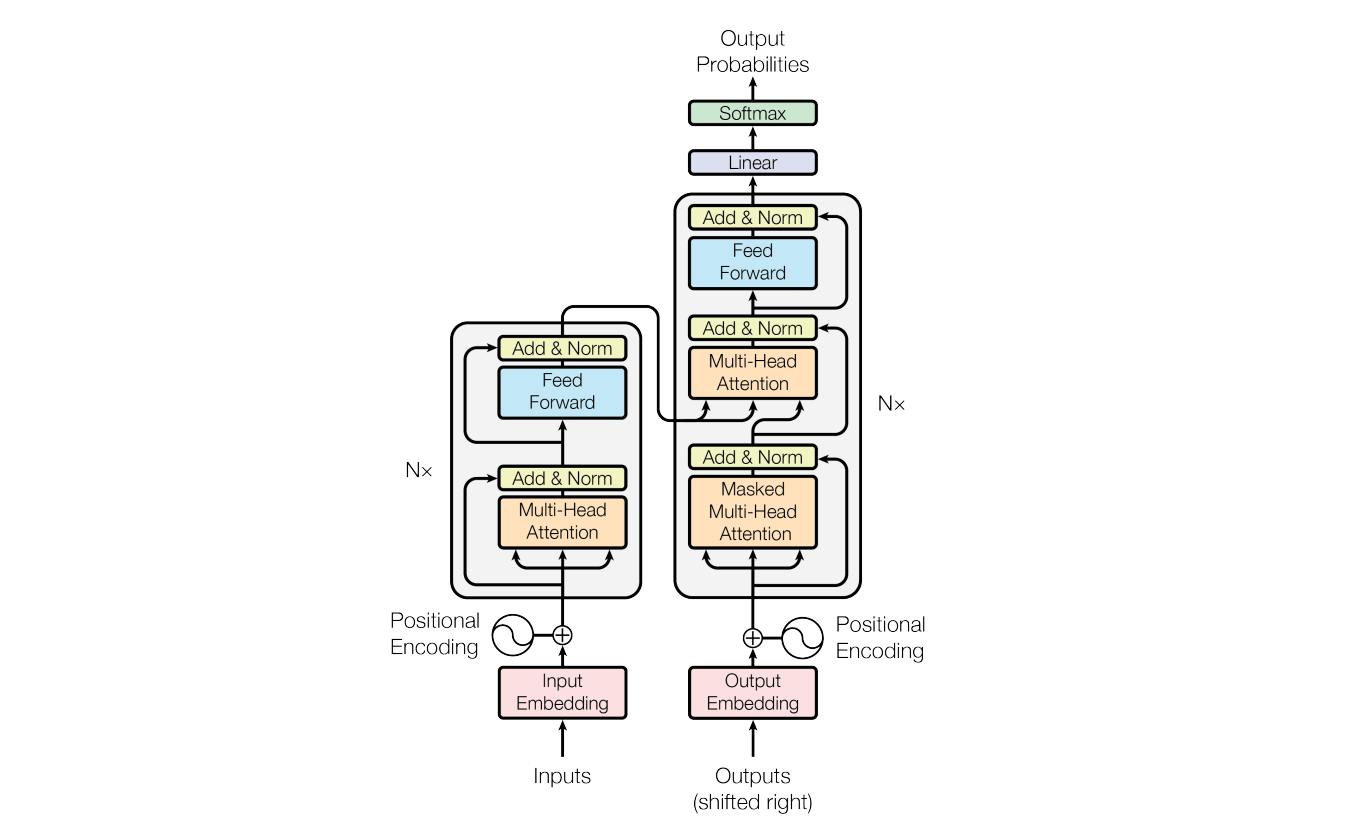
\includegraphics[width=1.0\textwidth]
    {images/domain_analysis/transformer_scheme.png}
    \caption{Схема архитектуры трансформера, взятая из оригинальной статьи.}
    \label{fig:transformer-scheme}
\end{figure}


Трансформер состоит из двух главных блоков (\autoref{fig:transformer-scheme}): трансформер кодировщик и трансформер декодировщик. Трансформер-кодировщик преобразует элементы входной последовательности в последовательность векторов той же длины. Каждый элемент последовательности учитывает связь со всеми остальными элементами, что обеспечивается механизмом внимания. В некоторых моделях, основанных на архитектуре трансформера-кодировщика, например BERT\cite{bert}, к последовательности входных данных добавляется элемент ``CLS``, токен класса. Данный элемент служит для агрегации всей информации последовательности в один плотный вектор.

Трансформер-декодировщик используется для генерации выходной последовательности авторегрессионно, то есть пошагово. В этом режиме, за один шаг работы модели предсказывается один новый элемент на основе предыдущих. 

Для получения последовательности элементов из единого текста применяются методы токенизации. В ходе токенизации, текст разбивается на лексемы, кодируемые при помощи словаря в плотные векторы - токены (слово ``token`` в переводе с английского языка означает ``лексема``, однако поскольку термин ``токен`` в контексте моделей-трансформеров также означает плотный вектор обрабатываемой последовательности, далее он будет использоваться именно в этом смысле).

\subsection{Механизм внимания}

Основа модели трансформер - механизм внимания. В моделях, основанных на архитектуре трансформер-кодировщик, используются механизмы самовнимания и многоглавого внимания. 

Механизм самовнимания вычисляет взаимное влияние элементов последовательности с помощью вычисления матрицы весов. С помощью матриц проекции $W_Q$, $W_K$, $W_V$ для векторов $X$ последовательности вычисляются матрицы ``запросов`` $q$, ``ключей`` $k$ и ``значений`` $v$:

$$
Q = X W_Q, \quad K = X W_K, \quad V = X W_V 
$$

Внимание вычисляется по следующей формуле:

$$
\text{Attention}(Q, K, V) = \text{softmax}\Big(\dfrac{QK^T}{\sqrt{\dim(K_0)}}\Big)V,
$$

где:

$$
\text{softmax}(x_i) = \dfrac{\exp(x_i)}{\sum\limits_{j=0}^{\dim(x)}\exp(x_j)}
$$

Таким образом, за счет вычисления квадратной матрицы весов внимания 

$$\text{softmax}\Big(\dfrac{QK^T}{\sqrt{\dim(K_0)}}\Big)$$

с размерностью, равной длине последовательности, каждый токен последовательности получает информацию о всех остальных токенах.

В многоглавом внимании механизм самовнимания разделяется на $h$ ``голов``, каждая из которых работает в подпространстве меньшей размерности:

$$
\text{MultiHead}(Q, K, V) = \text{Concat}(\text{head}_1, \cdots, \text{head}_h)W^O,
$$

где: 
\begin{itemize}
    \item $W^O$ - матрица проекции,
    \item $\text{head}_i = \text{Attention}(Q W_i^Q, K W_i^K, V W_i^V)$, а $W_i^Q$, $W_i^K$, $W_i^V$ - матрицы проекций в пространство меньшей размерности.
\end{itemize}

При использовании механизма многоглавого внимания, каждая ``голова`` фокусируется на разных аспектах данных параллельно, что позволяет моделировать более сложные зависимости.

\subsection{Применение модели типа Transformer для обработки изображений}

Изначально модели транформер применялись исключительно для обработки последовательных данных. Однако, поскольку данная архитектура обрабатывает каждый элемент параллельно, для обработки других типов данных их необходимо преобразовать в некоторое множество объектов. 

Наивный подход использования механизма самовнимания при обработке изображений подразумевает попиксельную токенизацию изображения. Для изображений большой размерности данный способ может привести к слишком большому размеру входной последовательности. Решение данной проблемы было предложено в работе Image Transformer \cite{image_transformer}, основанное на применении механизма внимания локально для разных групп пикселей. Однако такой подход исключает глобальное внимание.

С появлением Vision Transformer (ViT) \cite{vit} стало возможным эффективное применение моделей трансформеров для решения задач компьютерного зрения. 


\begin{figure}[H]
    \centering
    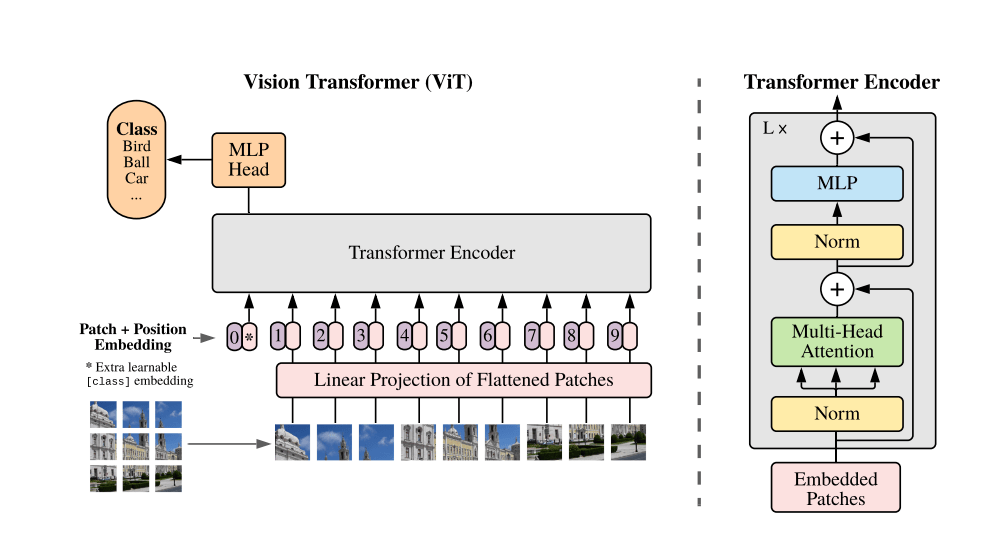
\includegraphics[width=1.0\textwidth]
    {images/domain_analysis/vit_scheme.png}
    \caption{Схема архитектуры Vision Transformer, взятая из оригинальной статьи.}
    \label{fig:vit-scheme}
\end{figure}


Модель ViT повторяет архитектуру (\autoref{fig:vit-scheme}) трансформера-кодировщика, однако заменяет процесс токенизации. В Vision Transformer токенизация реализуется посредством разбиения входного изображения на фиксированные по размеру и непересекающиеся между собой части - патчи (чаще всего, размером 16 на 16 пикселей). После разбиения, каждый патч выпрямляется в вектор и проецируется в пространство определенной размерности. 

Поскольку под термином ``токен`` рассматривается плотный вектор обрабатываемой последовательности, под термином ``токенизация`` будет далее подразумеваться процесс преобразования исходных данных в набор (множество) плотных векторов.

\subsection{Преимущества архитектуры Transformer}

Модели архитектуры трансформер обладают значительными преимуществами перед другими архитектурами:

\begin{itemize}
    \item В отличие от сверточных нейронных сетей, которые обрабатывают локальные паттерны, трансформеры анализируют глобальные зависимости через механизм самовнимания \cite{transformer}.
    \item Архитектура трансформер адаптирована для параллельных вычислений на графических ускорителях \cite{transformer}.
    \item Увеличение количества параметров модели позволяет значительно улучшить качество моделей \cite{gpt2}.
\end{itemize}

\subsection{Недостатки архитектуры Transformer}

Однако, несмотря на все свои преимущества, модель Transformer обладает значительным недостатком. Из-за размерности матрицы весов внимания, вычислительная сложность, а также требуемая память квадратично зависят от длины последовательности \cite{transformer_computation_complexity}.

Эта проблема также касается и обработки изображений. При обработке изображений большой размерности необходимо обрабатывать последовательности большой длины.

\subsection{Выводы по главе 1}
Архитектура трансформер, изначально разработанная для решения задач обработки естественного языка, была успешно адаптирована для обработки изображений благодаря Vision Transformer. Это позволило использовать преимущества модели транформер для обработки изображений. Однако ключевые проблемы трансформеров — квадратичная сложность вычислений механизма самовнимания и квадратичная память не были решены. Эти проблемы могут стать критичными при обработке изображений большого разрешения или нескольких изображений одновременно (например, кадров видео).
